\FloatBarrier
\section{Stage 4: End-to-end measurement and evaluation}
\subsection{Why whole-record NMSE, with MAE as an alternative}
\label{sec:r41}
I retain $ D=\operatorname{mean}[(\widehat x-u)^2]$ and
$ d=D/P_u $, $ P_u=\MReferencePower $, over all 96000 original positions.
The definition measures full-record squared reconstruction error
relative to the original reference power.
Appendix~\ref{app:metrics} derives the common definitions, bias identity,
MAE/RMSE relation and dB conventions. NMSE is dimensionless, lower is
better and it can exceed one; amplitude gain, timing and endpoints are
not fitted or trimmed. Centred variance alone would hide fixed bias.

MAE is a genuinely different loss; RMSE is a monotone transformation of
per-record MSE. Figure~\ref{fig:r41-ranking} shows why the choice matters:
diffuse error has $(D,\mathrm{MAE})=(0.01,0.1)$, sparse large errors
$(0.04,0.02)$. MAE prefers the latter, NMSE the former.
Natural-binary MSB errors are $2^{13}$ times the amplitude of LSB errors
at 14 bit ($2^{26}$ in squared error), supporting a loss sensitive to
large corruption. These local ratios do not determine total NMSE.

\begin{figure}[htbp]
 \centering
 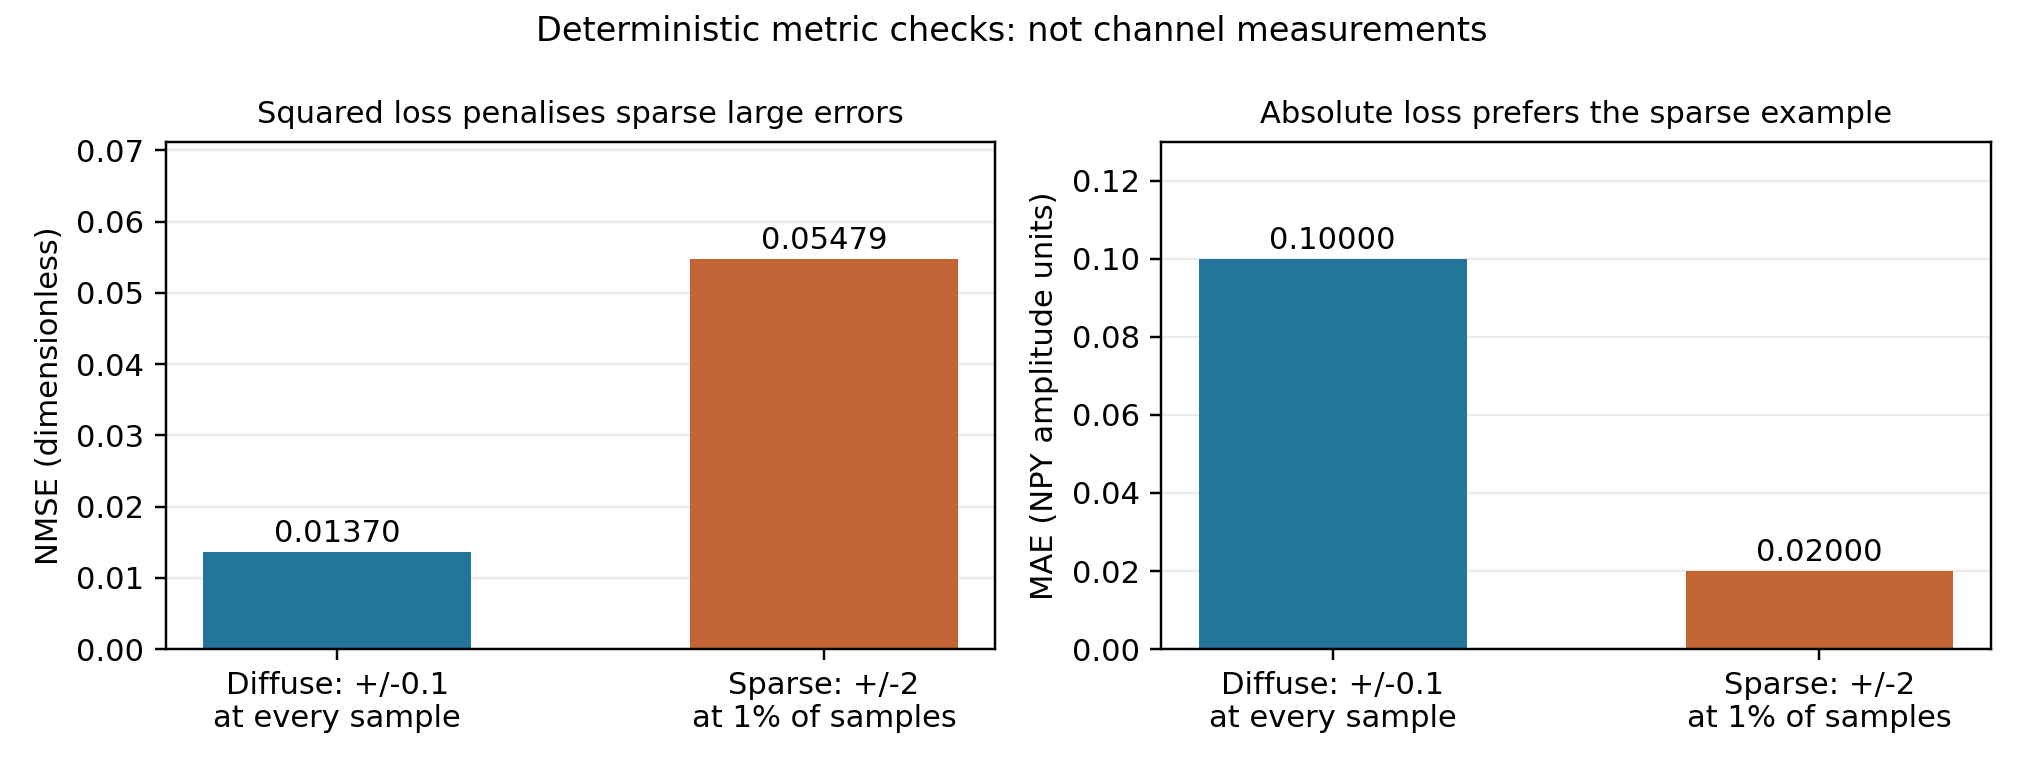
\includegraphics[width=.76\linewidth]{images/r41_metric_ranking.png}
 \caption{Declared full-grid metric counterexamples. NMSE favours diffuse small error, MAE the sparse large error. Axes retain their different units; this is not a stochastic channel experiment.}
 \label{fig:r41-ranking}
\end{figure}

MAE remains a diagnostic; neither metric is claimed as perceptual quality
\citep{wang2009mse}.
Correlation alone is insufficient: $\widehat x=2u $ has correlation one
but NMSE one. Likewise exact bit delivery retains upstream waveform
error. For repeated records I distinguish $-10\log_{10}\bar d $ from
the mean of individual dB ratios. Seven semantic checks/221 independent
assertions and the saved R3 examples verify these interpretations.
